% Options for packages loaded elsewhere
\PassOptionsToPackage{unicode}{hyperref}
\PassOptionsToPackage{hyphens}{url}
%
\documentclass[
]{article}
\usepackage{lmodern}
\usepackage{amsmath}
\usepackage{ifxetex,ifluatex}
\ifnum 0\ifxetex 1\fi\ifluatex 1\fi=0 % if pdftex
  \usepackage[T1]{fontenc}
  \usepackage[utf8]{inputenc}
  \usepackage{textcomp} % provide euro and other symbols
  \usepackage{amssymb}
\else % if luatex or xetex
  \usepackage{unicode-math}
  \defaultfontfeatures{Scale=MatchLowercase}
  \defaultfontfeatures[\rmfamily]{Ligatures=TeX,Scale=1}
\fi
% Use upquote if available, for straight quotes in verbatim environments
\IfFileExists{upquote.sty}{\usepackage{upquote}}{}
\IfFileExists{microtype.sty}{% use microtype if available
  \usepackage[]{microtype}
  \UseMicrotypeSet[protrusion]{basicmath} % disable protrusion for tt fonts
}{}
\makeatletter
\@ifundefined{KOMAClassName}{% if non-KOMA class
  \IfFileExists{parskip.sty}{%
    \usepackage{parskip}
  }{% else
    \setlength{\parindent}{0pt}
    \setlength{\parskip}{6pt plus 2pt minus 1pt}}
}{% if KOMA class
  \KOMAoptions{parskip=half}}
\makeatother
\usepackage{xcolor}
\IfFileExists{xurl.sty}{\usepackage{xurl}}{} % add URL line breaks if available
\IfFileExists{bookmark.sty}{\usepackage{bookmark}}{\usepackage{hyperref}}
\hypersetup{
  pdftitle={Informe},
  hidelinks,
  pdfcreator={LaTeX via pandoc}}
\urlstyle{same} % disable monospaced font for URLs
\usepackage[margin=1in]{geometry}
\usepackage{graphicx}
\makeatletter
\def\maxwidth{\ifdim\Gin@nat@width>\linewidth\linewidth\else\Gin@nat@width\fi}
\def\maxheight{\ifdim\Gin@nat@height>\textheight\textheight\else\Gin@nat@height\fi}
\makeatother
% Scale images if necessary, so that they will not overflow the page
% margins by default, and it is still possible to overwrite the defaults
% using explicit options in \includegraphics[width, height, ...]{}
\setkeys{Gin}{width=\maxwidth,height=\maxheight,keepaspectratio}
% Set default figure placement to htbp
\makeatletter
\def\fps@figure{htbp}
\makeatother
\setlength{\emergencystretch}{3em} % prevent overfull lines
\providecommand{\tightlist}{%
  \setlength{\itemsep}{0pt}\setlength{\parskip}{0pt}}
\setcounter{secnumdepth}{-\maxdimen} % remove section numbering
\usepackage{booktabs}
\usepackage{longtable}
\usepackage{array}
\usepackage{multirow}
\usepackage{wrapfig}
\usepackage{float}
\usepackage{colortbl}
\usepackage{pdflscape}
\usepackage{tabu}
\usepackage{threeparttable}
\usepackage{threeparttablex}
\usepackage[normalem]{ulem}
\usepackage{makecell}
\usepackage{xcolor}
\usepackage{amsmath}
\usepackage{caption}
\ifluatex
  \usepackage{selnolig}  % disable illegal ligatures
\fi

\title{Informe}
\author{}
\date{\vspace{-2.5em}}

\begin{document}
\maketitle

\hypertarget{introducciuxf3n}{%
\section{Introducción}\label{introducciuxf3n}}

A partir del año 2006, se llevó a cabo en Chile una serie de protestas
exigiendo reformas educativas. Dichas protestas fueron conocidas como
``Revolución de los pingüinos'', debido al uniforme escolar que se
utiliza en el país. Entre sus principales demandas se encontraba
prohibir el lucro en la educación privada y que el Estado brinde
educación pública, gratuita y de calidad (Fuente: BBC). Fruto de estas
protestas, en el año 2011 se crea la Agencia de Calidad de la Educación.
Este servicio público tiene como objetivo ``evaluar, informar y orientar
al sistema educativo para contribuir al mejoramiento de la calidad y
equidad de las oportunidades educativas de todos los estudiantes de
Chile'' (Fuente: Agencia de Calidad de la Educación).

Con respecto al primer objetivo, se puede mencionar que en Chile se
realizan diferentes pruebas para medir los aprendizajes en diversas
áreas curriculares como, por ejemplo, Compresión de Lectura, Matemática
o Ciencias Naturales. Algunas de estas evaluaciones pueden ser
nacionales, como el Simce, o parte de estudios internacionales como las
pruebas PISA, PIRLS, TIMSS, ERCE, entre otras.

De esta manera, se utilizarán las evaluaciones internacionales para
medir la calidad en educación en el país, a través del tiempo. Por ende,
con estas pruebas, además, se podrá determinar el impacto en reformas en
educación, medido a través del gasto público en este sector. Pues para
un gobierno que debe atender las necesidades de todo un país, no sólo
educación, es importante invertir eficientemente el dinero.

En este informe se investigará la relación entre los resultados de las
pruebas internacionales PISA y el gasto en educación en Chile entre los
años 2001 y 2018. Para ello se analizarán datos sobre los resultados en
las distintas áreas medidas en esa evaluación y sobre el gato público en
educación.

El informe contiene cuatro secciones. En la primera parte, se detallarán
las pruebas PISA, en particular, las áreas de conocimiento que evalúan y
cómo se interpretan los resultados obtenidos. En la segunda sección, se
mostrarán, brevemente, los datos utilizados. Además, se explicará las
metodologías que se utilizaron para el desarrollo del informe. Luego, se
presentarán los resultados obtenidos a partir del análisis, tanto
descriptivo como regresión. Por último, en la conclusión, se realizará
una proyección para futuras pruebas PISA.

\hypertarget{antecedentes}{%
\section{Antecedentes}\label{antecedentes}}

\hypertarget{pisa}{%
\subsubsection{PISA}\label{pisa}}

El programa para la Evaluación Internacional de Alumnos de la OCDE,
conocido como PISA por sus siglas en inglés (Programme for International
Student Assessment) es un proyecto que tiene por objetivo evaluar la
formación de los alumnos cuando llegan al final de la etapa de enseñanza
obligatoria a los 15 años.

Para cumplir este objetivo, PISA realiza pruebas cada tres años. Éstas
cubren las áreas de lectura, matemáticas y competencias científicas. El
enfásis de la evaluación está puesto en el dominio de los procesos, el
entendimiento de los conceptos y la habilidad de actuar o funcionar en
varias situaciones dentro de cada dominio.

Los resultados son reportados como puntajes y niveles de desempeño. Se
establecen escalas para los puntajes para cada asignatura, diseñadas
para mostrar las compentencias generales. Además, en teoría no existe un
puntaje máximo o mínimo, pues los resultados se escalan para ajustarse a
distribuciones aproximadamente normales, con media 500 puntos y
desviación estándar de 100 puntos aproximadamente.\footnote{Extraído
  desde \href{https://www.oecd.org/pisa/pisafaq/}{PISA}}. Luego de
calificar al alumno, su puntaje se puede ubicar en una escala adecuada,
denominada niveles de desempeño. Para matemática y ciencias se
establecen seis niveles de logro y para lectura son siete.

Finalmente, las pruebas PISA no entregan información colectiva para
todas las asignaturas combinadas, por el contrario, da una puntación por
cada área. Además, se suele utilizar el puntaje medio por asignatura
para clasificar a los países. Sin embargo, no es posible asignar una
clasificación exacta a cada país en función del puntaje medio, pues se
utiliza una muestra (entre 4.500 y 10.000 estudiantes por país) y debido
a la inceridumbre estadística solo es posible obtener un rango de
posiciones (límite inferior o superior del ranking) donde se puede
encontrar un país.

\hypertarget{datos}{%
\section{Datos}\label{datos}}

Para este informe se utilizaron datos de cuatro bases diferentes
disponibles desde The World Bank\footnote{Extraído desde
  \href{https://datatopics.worldbank.org/education/}{The World Bank}}.
\textbf{Dos de ellas corresponden a información sobre gastos y
resultados en pruebas internacionales en Chile, y las demás a
información sobre América del Sur}. El primer archivo
\texttt{expenditures\_explanation.csv} contiene datos sobre diferentes
variables relacionadas con gastos en educación en Chile. Para este
informe se utilizaron las variables ``Gastos en educación como
porcentaje del gasto público total'', además de ``Gasto público en
educación secundaria inferior como porcentaje del PIB''. También se
considera en el informe otros niveles educacionales como primaria,
preescolar, secundaria y secundaria superior.

El segundo archivo, llamado \texttt{learning\_outcomes.csv}, contiene
datos sobre los puntajes obtenidos en el país en diferentes pruebas
internacionales, como las evaluaciones LLECE, PIIAC, TIMSS, PISA, entre
otras. Para este trabajo se utizaron los puntajes PISA, específicamente,
el rendimiento medio en la escala de las áreas de matemática, lectura y
ciencia.

Para ambas bases de datos, se transponen las columnas que representan
los años, y se sintetiza la información en dos columnas, la primera con
los años y la segunda con la información que posee la dicha celda.
Finalmente, se seleccionan las variables de interés y se filtran los
datos para que no existan celdas sin valores.

\captionsetup[table]{labelformat=empty,skip=1pt}
\begin{longtable}{ll}
\toprule
variable & descripcion \\ 
\midrule
Country Name & País \\ 
Country Code & Código país \\ 
Series & Variable \\ 
Series Code & ID variable \\ 
puntaje\_anio & Puntaje \\ 
year & Año \\ 
 \bottomrule
\end{longtable}
\captionsetup[table]{labelformat=empty,skip=1pt}
\begin{longtable}{ll}
\toprule
variable & descripcion \\ 
\midrule
Country Name & País \\ 
Country Code & Código país \\ 
Series & Variable \\ 
Series Code & ID variable \\ 
gasto\_anio & Puntaje \\ 
year & Año \\ 
 \bottomrule
\end{longtable}

\hypertarget{datos-sudamuxe9rica}{%
\subsubsection{Datos sudamérica}\label{datos-sudamuxe9rica}}

Los datos que se utilizaron de los archivos
\texttt{expenditures\_sa.csv} y \texttt{learning\_outcomes\_sa.csv}.
Éstas contienen información sobre los gatos en educación y resultados de
pruebas internacionales, respectivamente, por país. Para obtener los
resultados, primero en ambas tablas se transponen las columnas que
poseen los años, donde se obtienen dos columnas una que representa el
año y otra que posee el valor de dicha variable. Luego se filtran ambas
tablas según las variables de interés. Para los gastos corresponde a la
variable ``Gasto como porcentaje del PIB'' y para los resultados el
puntaje promedio en las prueba PISA en las áreas de matemática, lectura
y ciencias. Después, se filtran las columnas para que no tenga valores
nulos, se unen las tablas según país y año,y se seleccionan las columnas
de interés. Finalmente, las variables de los puntajes se transponen para
que los valores están en las columnas.

\captionsetup[table]{labelformat=empty,skip=1pt}
\begin{longtable}{ll}
\toprule
variable & descripcion \\ 
\midrule
Country Name & País \\ 
Country Code & Código país \\ 
anio & Año \\ 
gasto\_educacion & Gasto educación \\ 
matematica & Puntaje Matemática \\ 
lectura & Puntaje Lectura \\ 
ciencia & Puntaje Ciencia \\ 
 \bottomrule
\end{longtable}

\hypertarget{desarrollo}{%
\section{Desarrollo}\label{desarrollo}}

\hypertarget{anuxe1lisis-descriptivo}{%
\subsection{Análisis descriptivo}\label{anuxe1lisis-descriptivo}}

Uno de los objetivos promovidos por la revolución pingüina fue la
calidad en la educación. Sin embargo, esta no es la unica demanda que el
gobierno tiene que atender. Como los recursos que posee el Estado son
limitados es importante utilizar eficientemente los recursos destinados
en cada sector.

Una forma de medir el dinero que destinado por parte del Estado a
educación es el gasto público en este sector como porcentaje del gasto
público total. Se utiliza esta variable, pues permite ver el cambio en
el gasto público sin considerar el gasto privado en este sector. Además,
permite comparar en diferentes años sin que sea afectado por el valor de
la moneda. En la siguiente figura podemos ver la evoluación de esta
variable.:

\begin{center}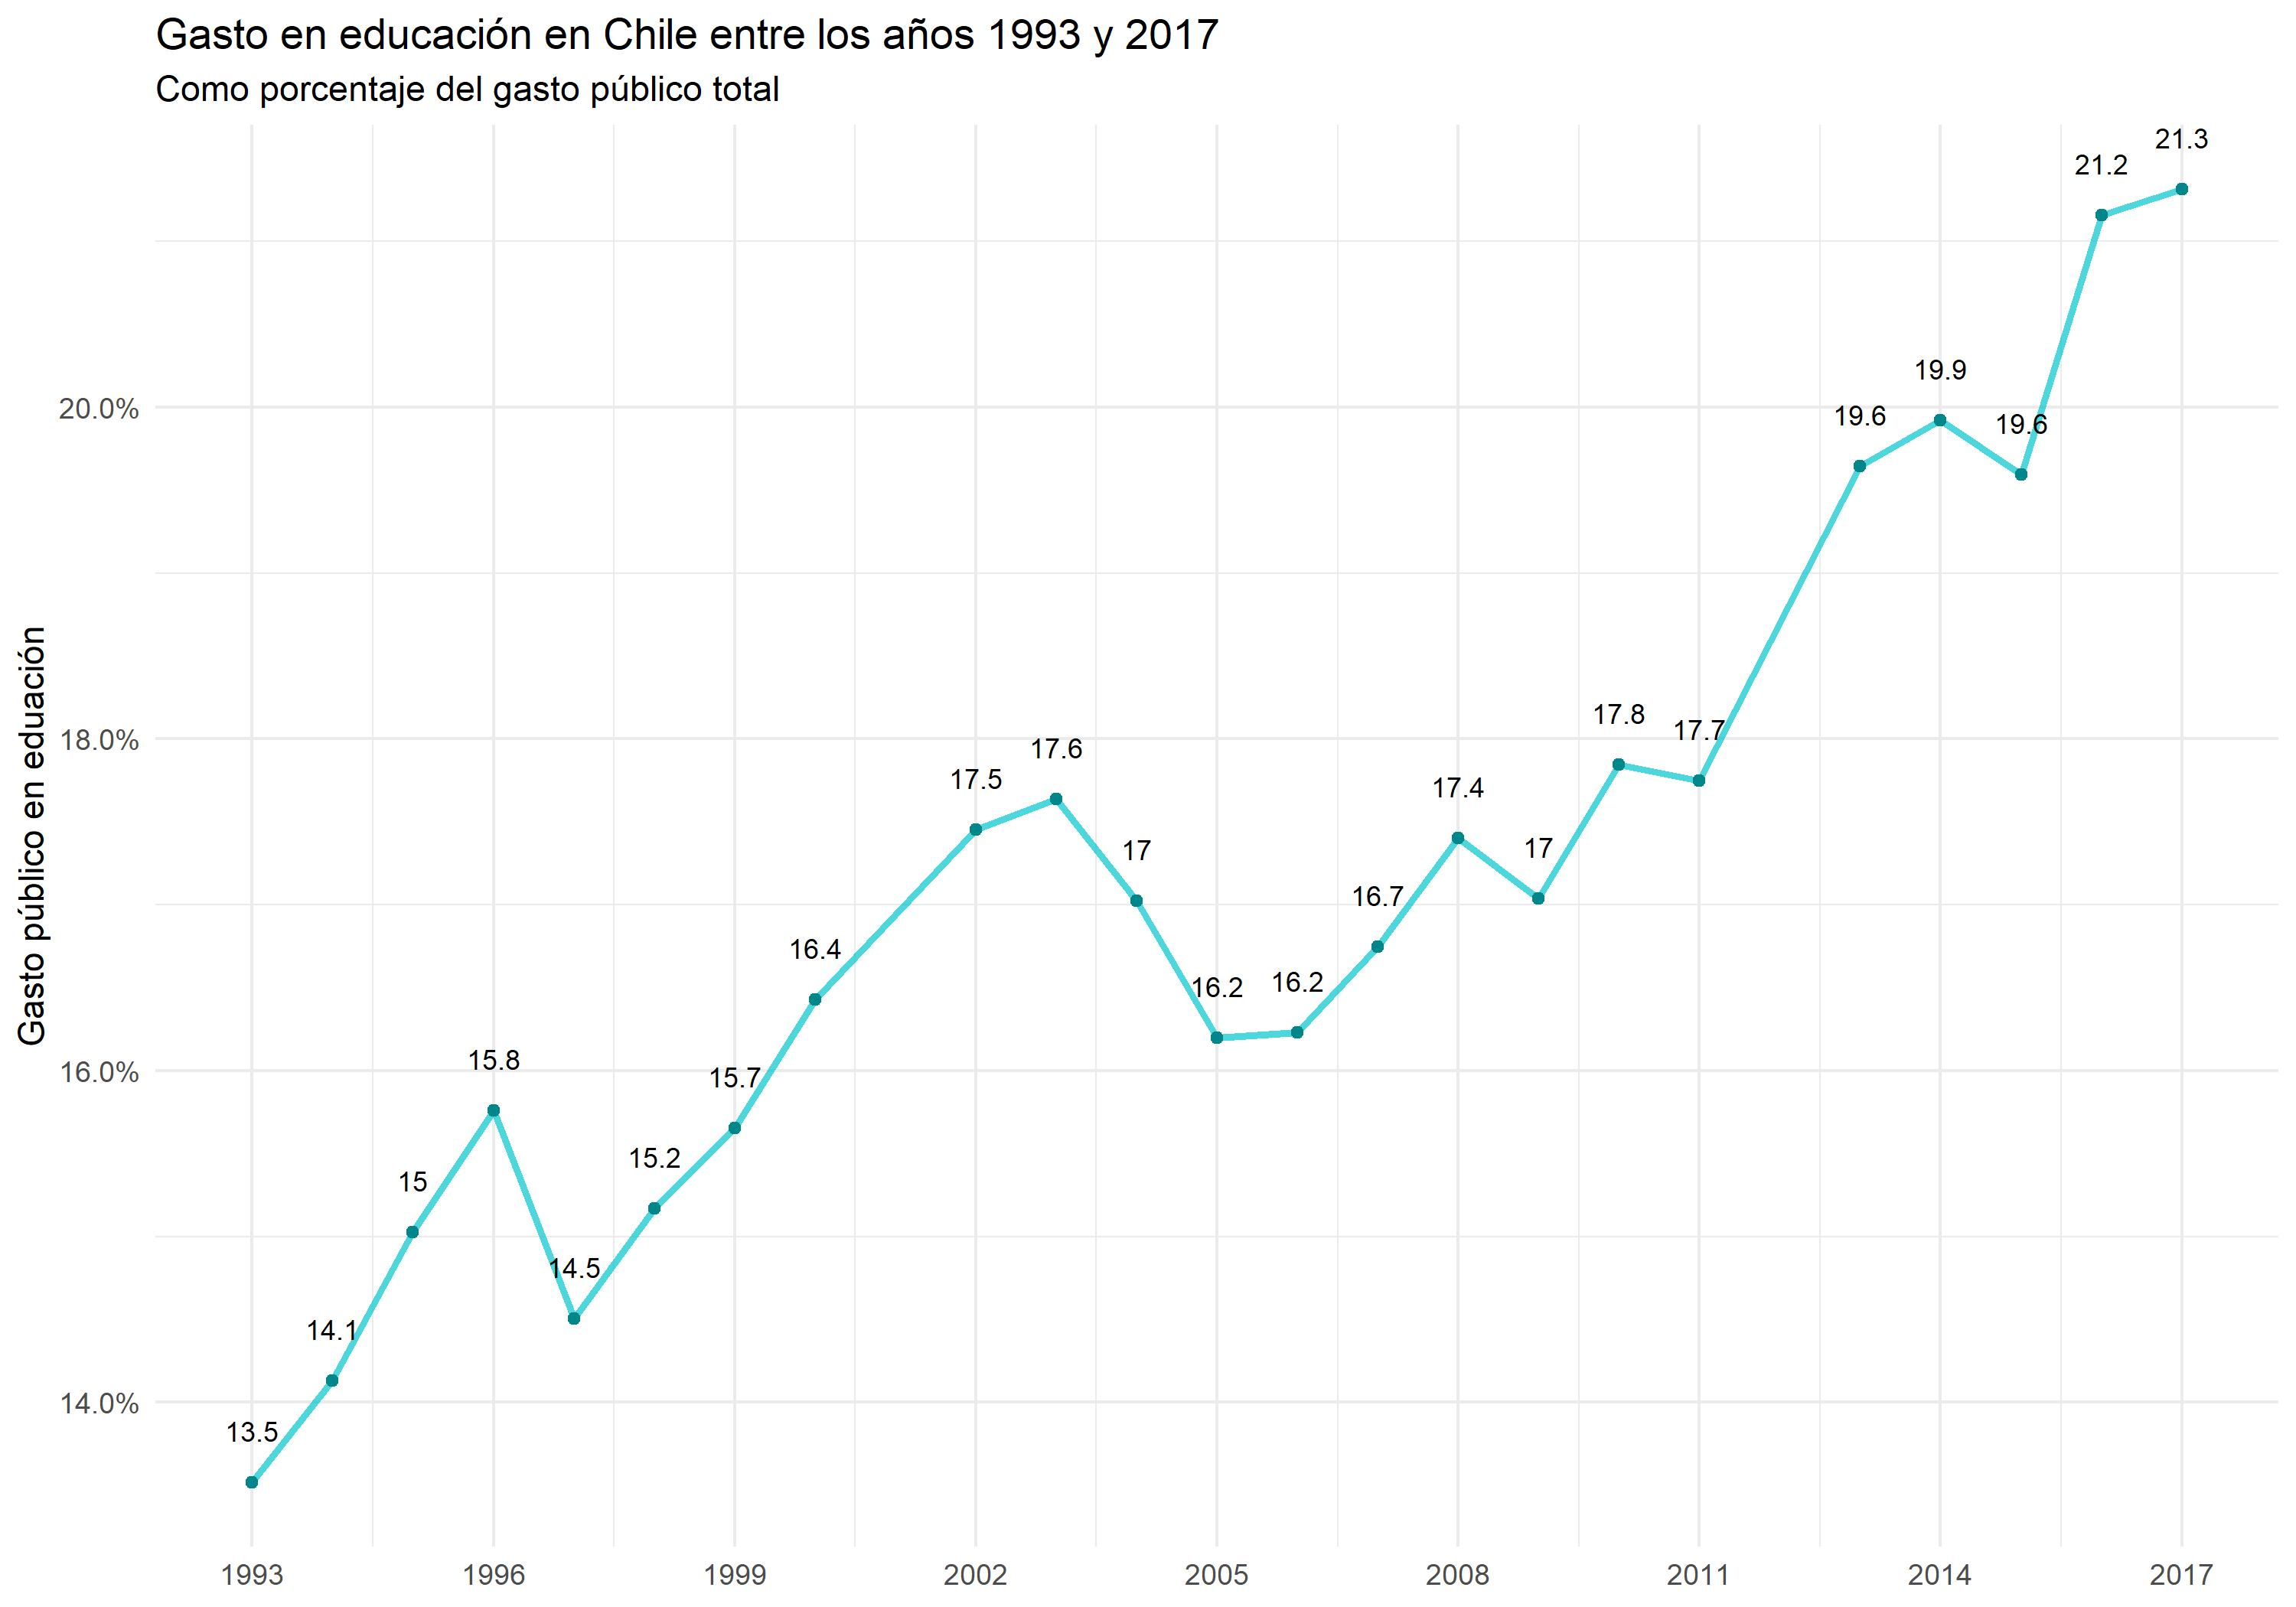
\includegraphics[width=0.85\linewidth]{C:/Users/56984/OneDrive/Documentos/Universidad/[2021-2] Sexto semestre/LET0010 - Habilidades Comunicativas para Estadísticos/Repositorio-LET0010/figuras/lineas_gasto-educacion_chile} \end{center}

En el gráfico anterior se puede apreciar que, en general, entre los años
1993 y 2017 ha aumentado el \textbf{gasto} en educación respecto a el
gasto público total. Además, es posible identificar una disminución del
gasto en esta área entre los años 2003 y 2006. Sin embargo, desde que
inició la ``Revolución Pingüina'', se puede advertir que el gasto vuelve
aumentar \textbf{llegando} a 21.3\% el año 2017. Lo que evidencia que
para el Estado ha adquirido mayor importancia la inversión en educación,
pues cada vez más ocupa una mayor proporción en el gasto público.

No obstante, con la variable anterior no se tiene informacion sobre qué
proporción del gasto público en esta área recibe cada nivel educacional,
es decir, no se puede determinar si se invierte más en educación
preescolar o secundaria. Para ello se utilizará el gasto en educación
como porcentaje del PIB, en los niveles preescolar, primaria y
secundaria. Así, se puede comparar la inversión en cada nivel para un
mismo año, como se observa en el siguiente gráfico siguiente gráfico:

\begin{center}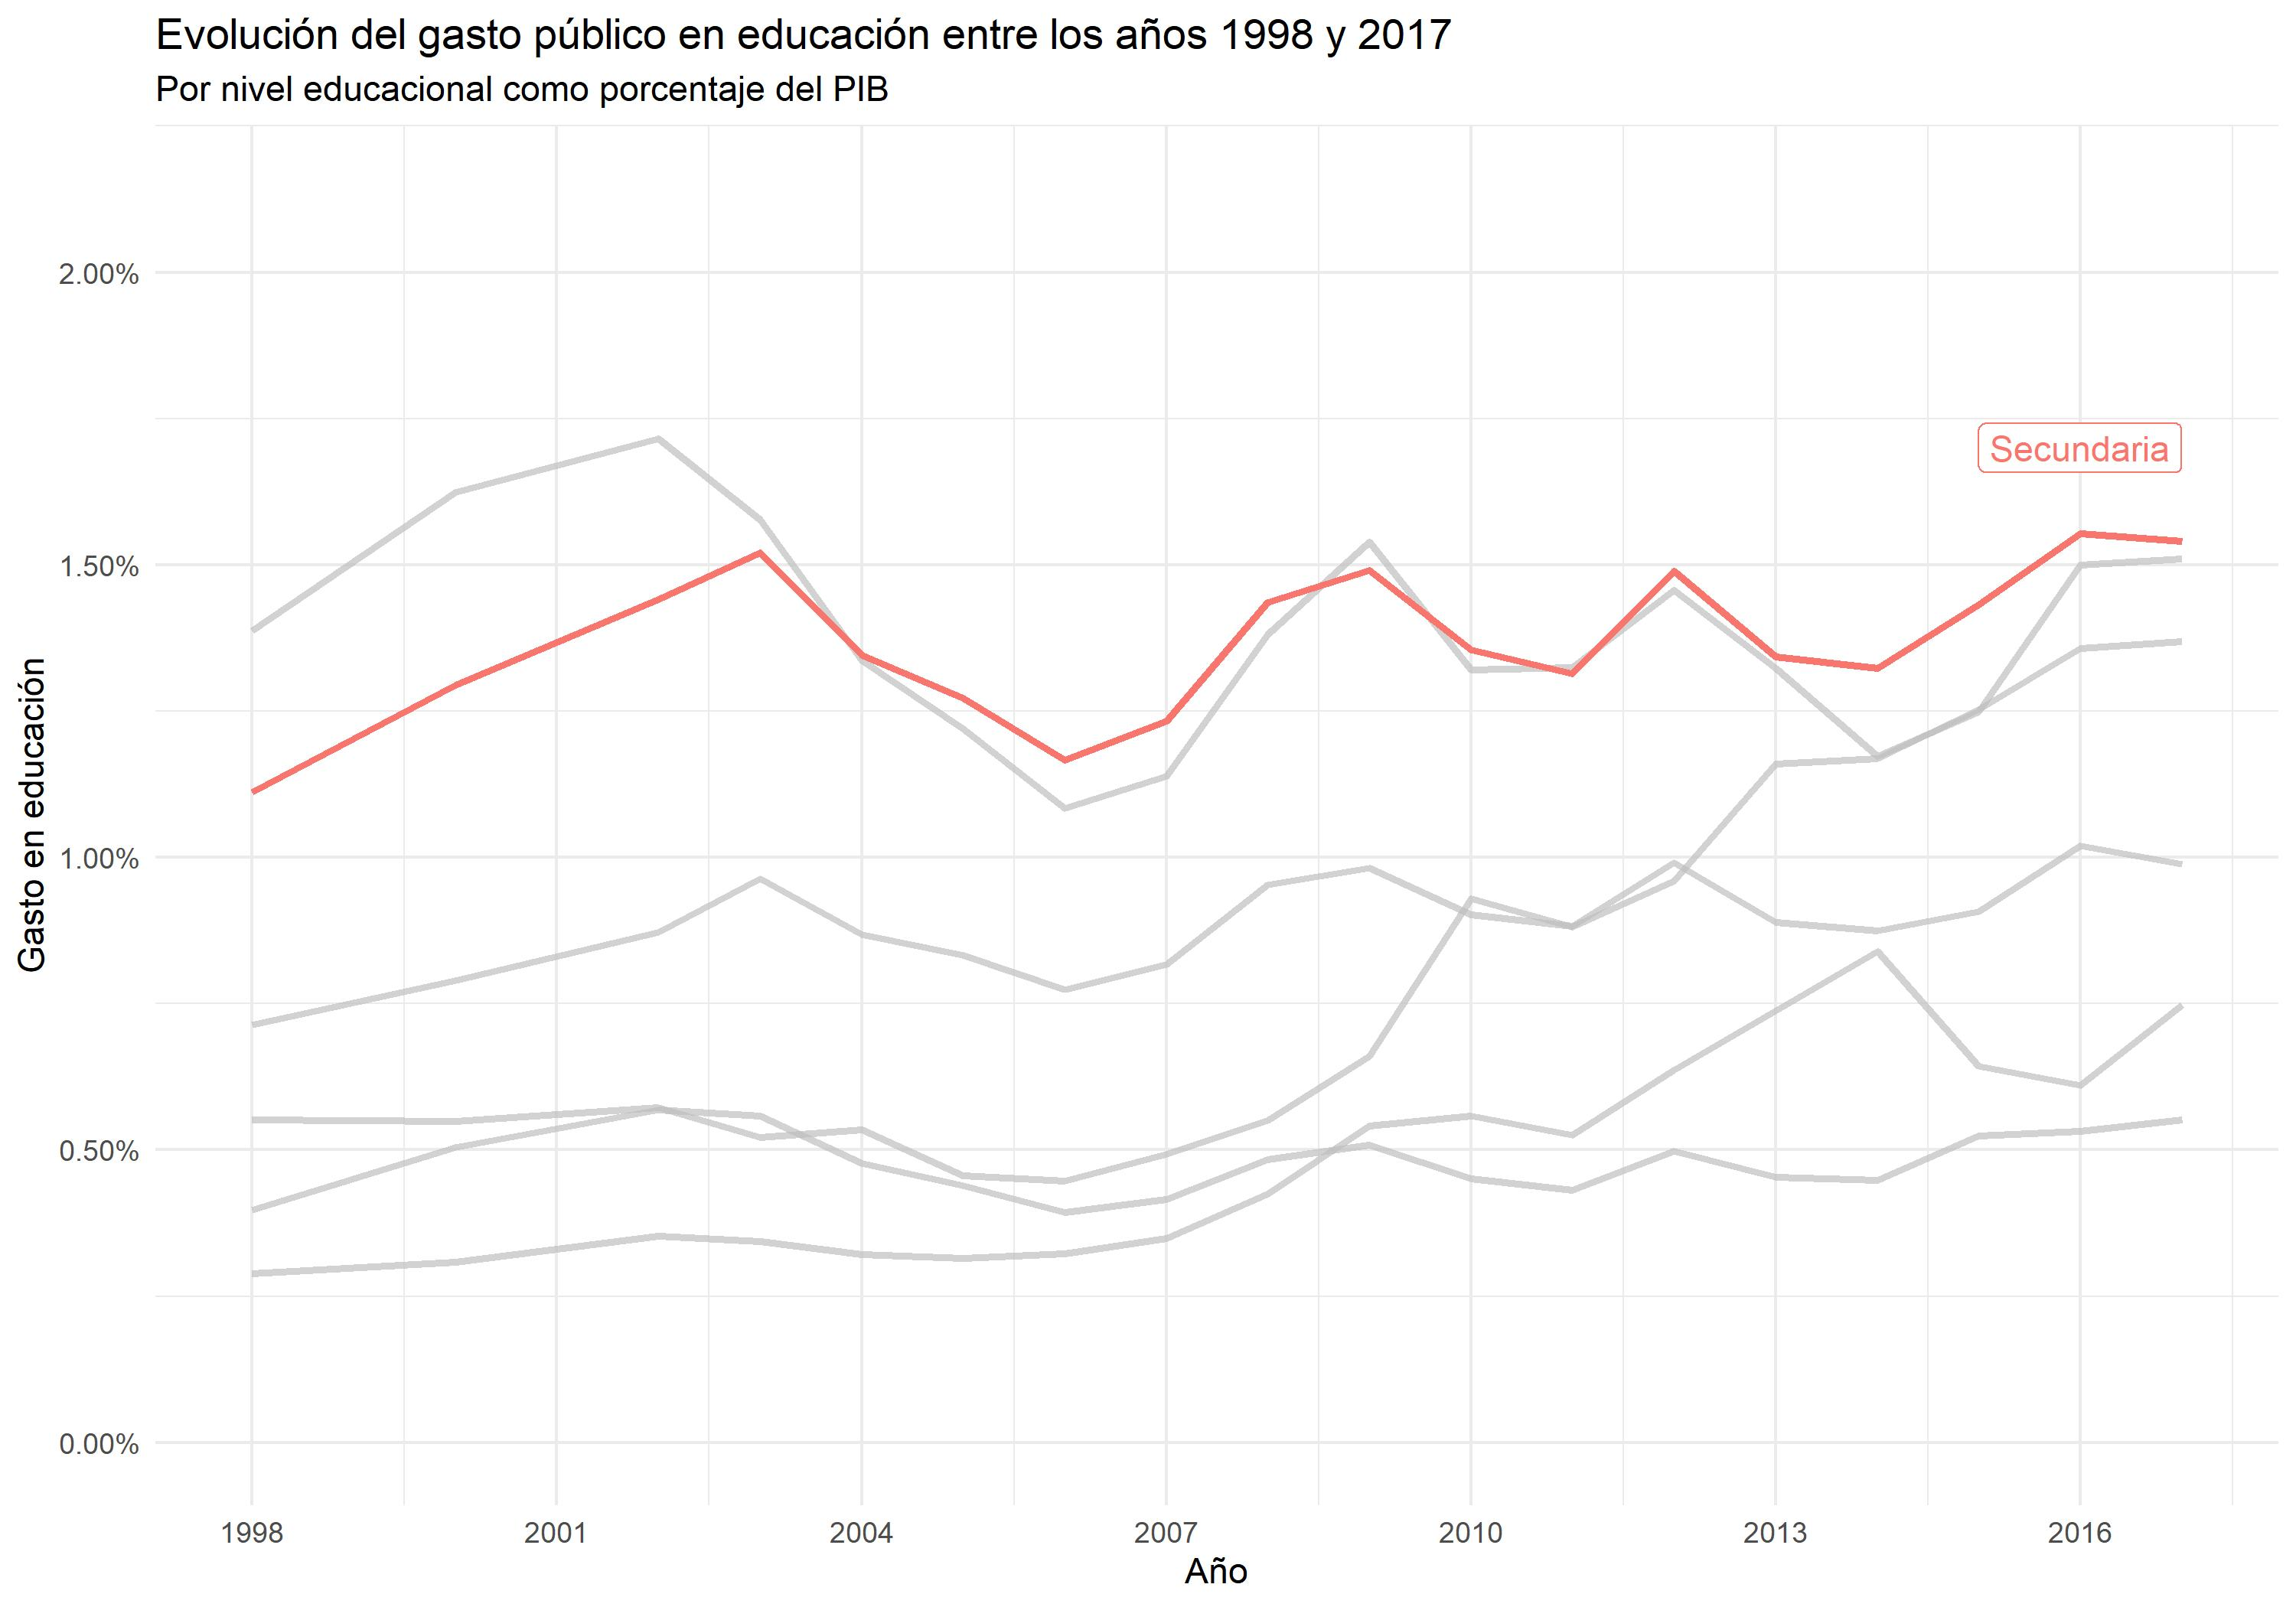
\includegraphics[width=0.85\linewidth]{C:/Users/56984/OneDrive/Documentos/Universidad/[2021-2] Sexto semestre/LET0010 - Habilidades Comunicativas para Estadísticos/Repositorio-LET0010/figuras/lineas_gasto-por-sector-educacion_chile} \end{center}

\textbf{En el gráfico anterior se observa que la educación secundaria ha
sido uno de los niveles donde más se ha invertido a través del tiempo.
además ésta oscila en el tiempo entorno 1,3\% del PIB. Entonces, ha
aumentado el gasto en educación como porcentaje el gasto público total,
además, el nivel de interés, es decir, la educación secundaria ha sido
uno de los que más se ha invertido en Chile en los últimos años.}

El análisis anterior permite concluir que en Chile la inversión pública
en educación ha aumentado. Sin embargo, ¿se verá reflejado este aumento
en mejoras en la calidad? Para medir esta variable existen diferentes
indicadores, en este informe en particular se medirá en términos del
aprendizaje y no se consideran otras \emph{variables} como la equidad o
asistencia escolar.

Para \emph{medir} los resultados en el aprendizaje se utilizarán los
datos de las pruebas PISA. Como se mencionó anteriormente estas
evaluaciones son estandarizadas y de gran importancia para los países
pertenecientes a la OCDE. Chile ha participado en todas las instancias
desde el año 2000. Para poder ver los cambios a través del tiempo, se
utiliza la media de los resultados en las pruebas por área de
conocimiento. Los resultados se muestran en la siguiente figura:

\begin{center}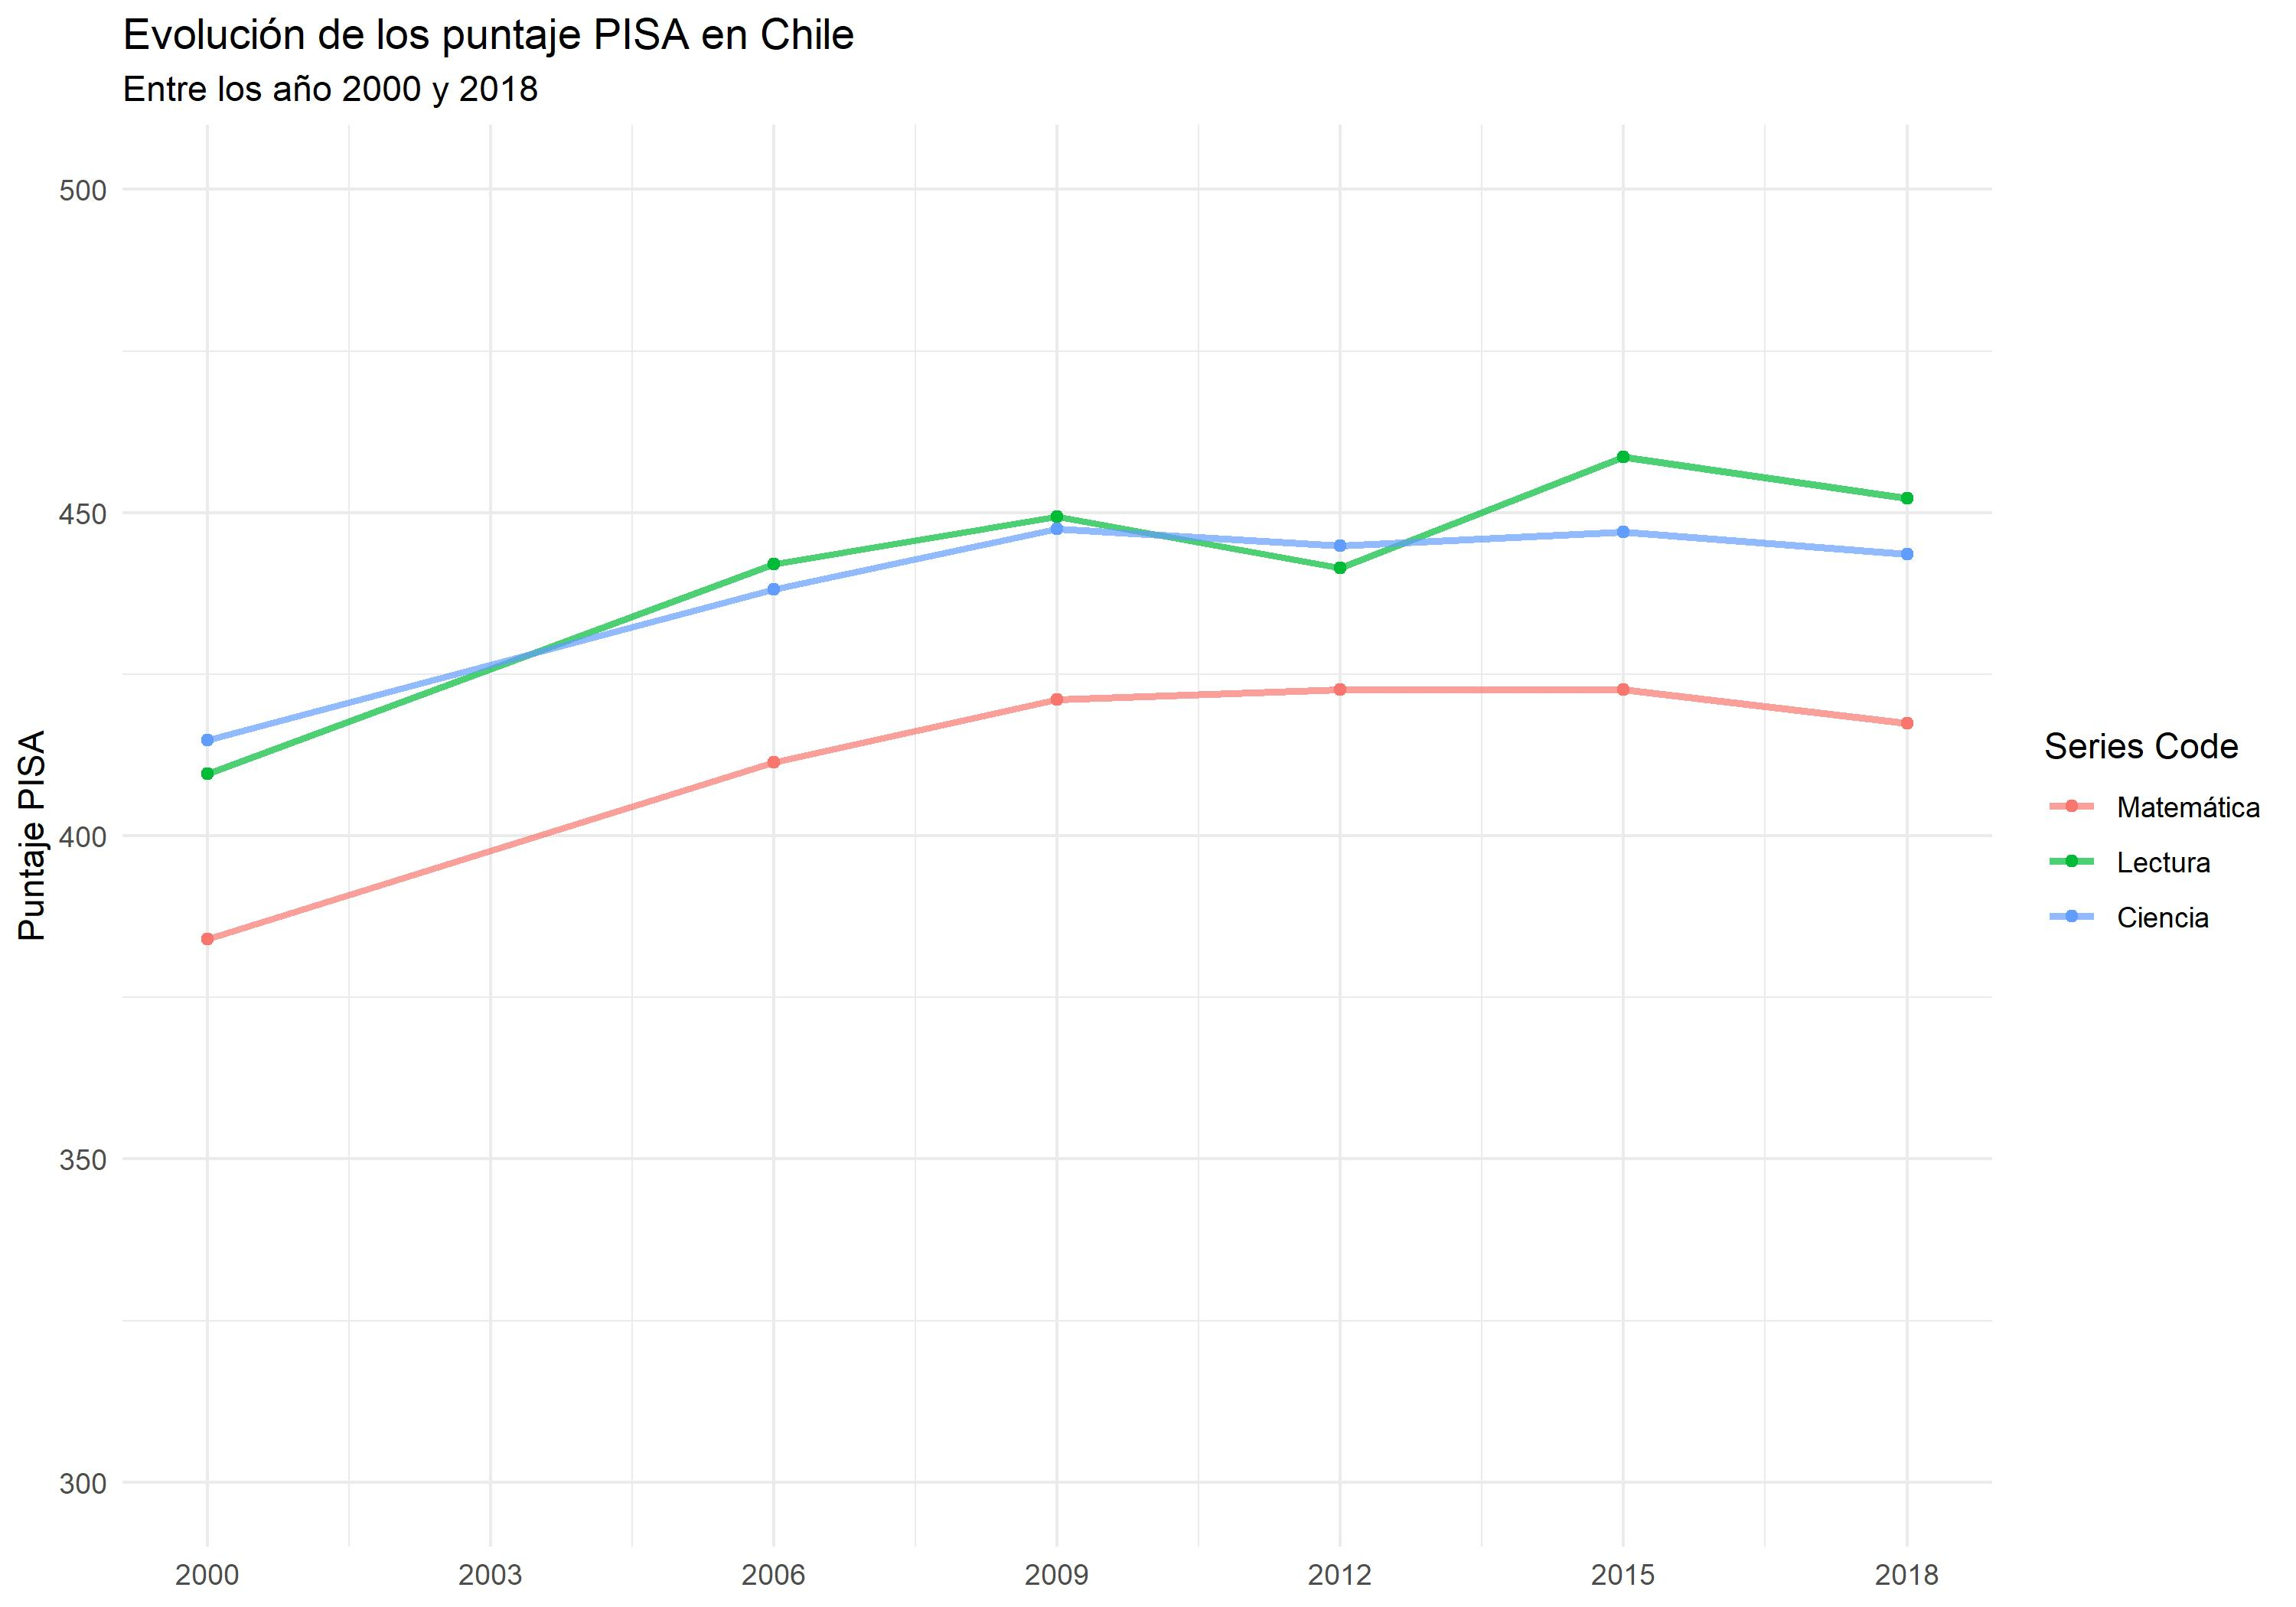
\includegraphics[width=0.85\linewidth]{C:/Users/56984/OneDrive/Documentos/Universidad/[2021-2] Sexto semestre/LET0010 - Habilidades Comunicativas para Estadísticos/Repositorio-LET0010/figuras/lineas_puntaje_pisa} \end{center}

En el figura anterior se observa que los puntajes han mejorado desde el
año 2000 hasta 2009. En el caso Ciencias y Matemática los resultados se
mantuvieron constantes. Para Lectura, los puntajes tuvieron variaciones
entre 2009 y 2015. En las tres categorias disminuyeron los puntajes del
2018, en comparación al año 2015. A partir de los anteriors sería
posible conlcuir que desde el año 2009 no se aprecian mejoras
significativas en el aprendizaje de los alumnos, puesto que la media por
área de conocimiento se ha mantenido o disminuido.

\hypertarget{anuxe1lisis-de-regresiuxf3n}{%
\subsection{Análisis de regresión}\label{anuxe1lisis-de-regresiuxf3n}}

Para analizar la relación entre el gasto público en educación y calidad
se utilizará la base de datos con información de América del Sur, pues
los datos disponibles en Chile no permitian realizar análisis de
regresión. Para este procedimiento, se utilizarán las variables gasto en
educación como porcentaje del PIB y la media de los resultados por país
y área de conocimiento.

En primer lugar se utilizará la correlación entre las descritas
anteriormente variables, pues la correlación mide el grado de asociasión
lineal entre éstas. A continuación se muestra la matriz de correlaciones

\captionsetup[table]{labelformat=empty,skip=1pt}
\begin{longtable}{lrrrr}
\toprule
 & gasto\_educacion & matematica & lectura & ciencia \\ 
\midrule
gasto\_educacion & 1.0000 & 0.0401 & 0.1024 & 0.0698 \\ 
matematica & 0.0401 & 1.0000 & 0.8497 & 0.9339 \\ 
lectura & 0.1024 & 0.8497 & 1.0000 & 0.9382 \\ 
ciencia & 0.0698 & 0.9339 & 0.9382 & 1.0000 \\ 
 \bottomrule
\end{longtable}

La tabla anterior muestra que entre la media de los puntajes PISA existe
una alta correlación. Sin embargo, con el gasto en educación existe una
muy baja correlación. Como se quiere investigar la relación entre
calidad de la educación y el gasto en este sector se utilizá análisis de
regresión simple como metodología, pues ésta permite explicar una
variable en función de otra. En este sentido, la variable respuesta será
el puntaje medio y como predictor el gasto en educación como porcentaje
del PIB. El ajuste del modelo se puede ver en la siguiente tabla

\captionsetup[table]{labelformat=empty,skip=1pt}
\begin{longtable}{lrrrr}
\toprule
coeficiente & valor estimado & error estándar & estadístico F & valor-p \\ 
\midrule
(Intercept) & 400.386 & 17.153 & 23.342 & $1.718 \times 10^{-18}$ \\ 
gasto\_educacion & 5.215 & 10.136 & 0.514 & $6.114 \times 10^{-1}$ \\ 
 \bottomrule
\end{longtable}

La tabla anterior evidencia que el modelo no es significativo.(\ldots)

\includegraphics{informe_files/figure-latex/unnamed-chunk-8-1.pdf}

\hypertarget{conclusiuxf3n}{%
\subsection{Conclusión}\label{conclusiuxf3n}}

\hypertarget{referencias}{%
\subsection{Referencias}\label{referencias}}

Richard Iannone, Joe Cheng and Barret Schloerke (2021). gt: Easily
Create Presentation-Ready Display Tables. R package version 0.3.1.
\url{https://CRAN.R-project.org/package=gt}

Wickham et al., (2019). Welcome to the tidyverse. Journal of Open Source
Software, 4(43), 1686, \url{https://doi.org/10.21105/joss.01686}

David Robinson, Alex Hayes and Simon Couch (2021). broom: Convert
Statistical Objects into Tidy Tibbles. R package version 0.7.9.
\url{https://CRAN.R-project.org/package=broom}

\end{document}
